\chapter{Introduction to NoSQL Injection}
This section outlines the concept of NoSQL injection and how it derives from conventional SQL injection. A definition of NoSQL injection is given along with a detailed analysis of the corresponding attacker models.

\section{From SQL to NoSQL Injection}
Injection attacks on relational databases represent the major web application vulnerability of the last decade. Thereby, the three tier architecture composed of client, server and database plays an important role. Since data obtained from the client can be arbitrary manipulated, input validation and sanitizing represent important principles for the the server-side. Otherwise, unvalidated input may find its way into sensitive operations, that cause injection vulnerabilities. In case unvalidated data is used to build database queries, an attacker is able to alter the SQL statement's structure. Suchlike vulnerabilities represent serious threats, especially due to the direct data access in combination with the Touring completeness of the injected SQL context.\\ 

This situation changed with the emerging generation of NoSQL databases. A variety of new query techniques was introduced next to SQL. For many databases, JSON-based or parameterized function calls replaced the conventional SQL approach. These simplified methods lead to a more straightforward database access and enabled unstructured data models. All the same, program logic moved from the database to the application layer due to functional limitations of the queries. Complex operations, such as data constraints or checks, that were previously executed directly on the database with SQL, have to be implemented within the application layer. Bypassing these logical constraints in order to achieve a certain database behavior constitutes an important aspect in the context of NoSQL injection. \\ 

Beside the query techniques, also the architecture of systems diversified with the emerged NoSQL databases. Relational databases are similar regarding their strengths and weaknesses, leading to a deployment in typical system structures, like the three tier model. In contrast to that, NoSQL databases discern in their focused area of application. Special requirements demand for tailored databases or even a combination of them. This leads to heterogeneous system landscapes deploying different databases and technology stacks for distinct purposes. Data exchange between multiple databases becomes an vital aspect that has to be managed. The resulting diversity of system designs as well as the data exchange between different data models has to be considered for the attack surface of NoSQL injection. All in all, NoSQL injection faces a much more diverse environment in contrast to conventional SQL injection.

\section{Definition of NoSQL Injection}

- and indeed the attacker models for NoSQL injection are much more diverse in comparison to conventional SQL injection
- also the processing logic is partly moved to the application layer
- bypasses become possible
- analyze the underlying problem of known and found injection attacks

\subsection{Common Attacker Model}

\begin{figure}[h]
\centering
  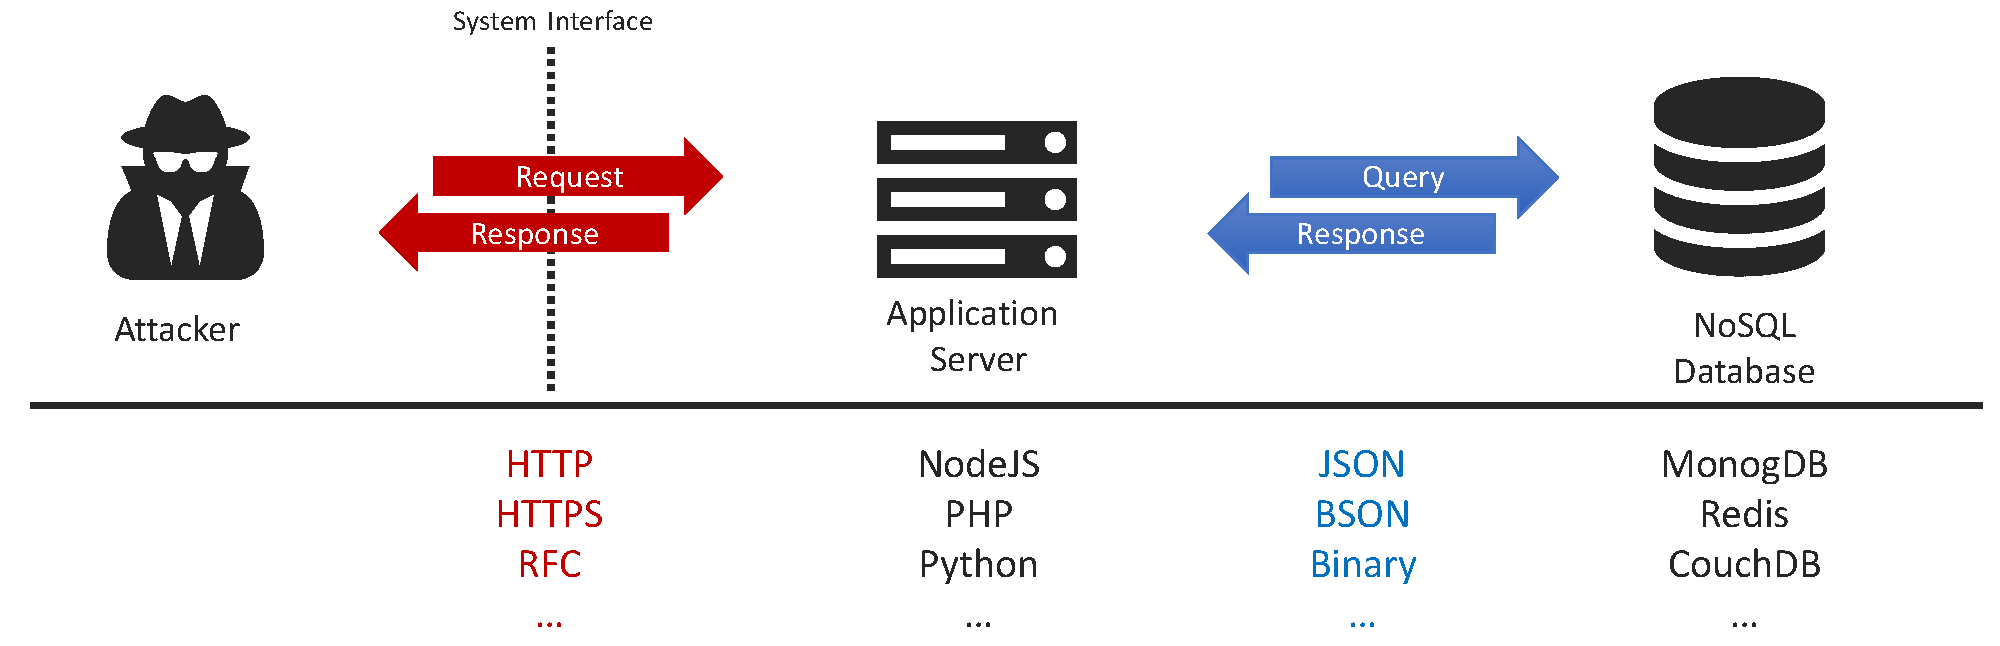
\includegraphics[width=1\linewidth]{Images/attacker_model_normal}
  \caption{Common attacker model for NoSQL injection}
  \label{fig:normalAttackerModel}
\end{figure}

% Objective

\subsection{Extended Attacker Model}

\begin{figure}[h]
\centering
  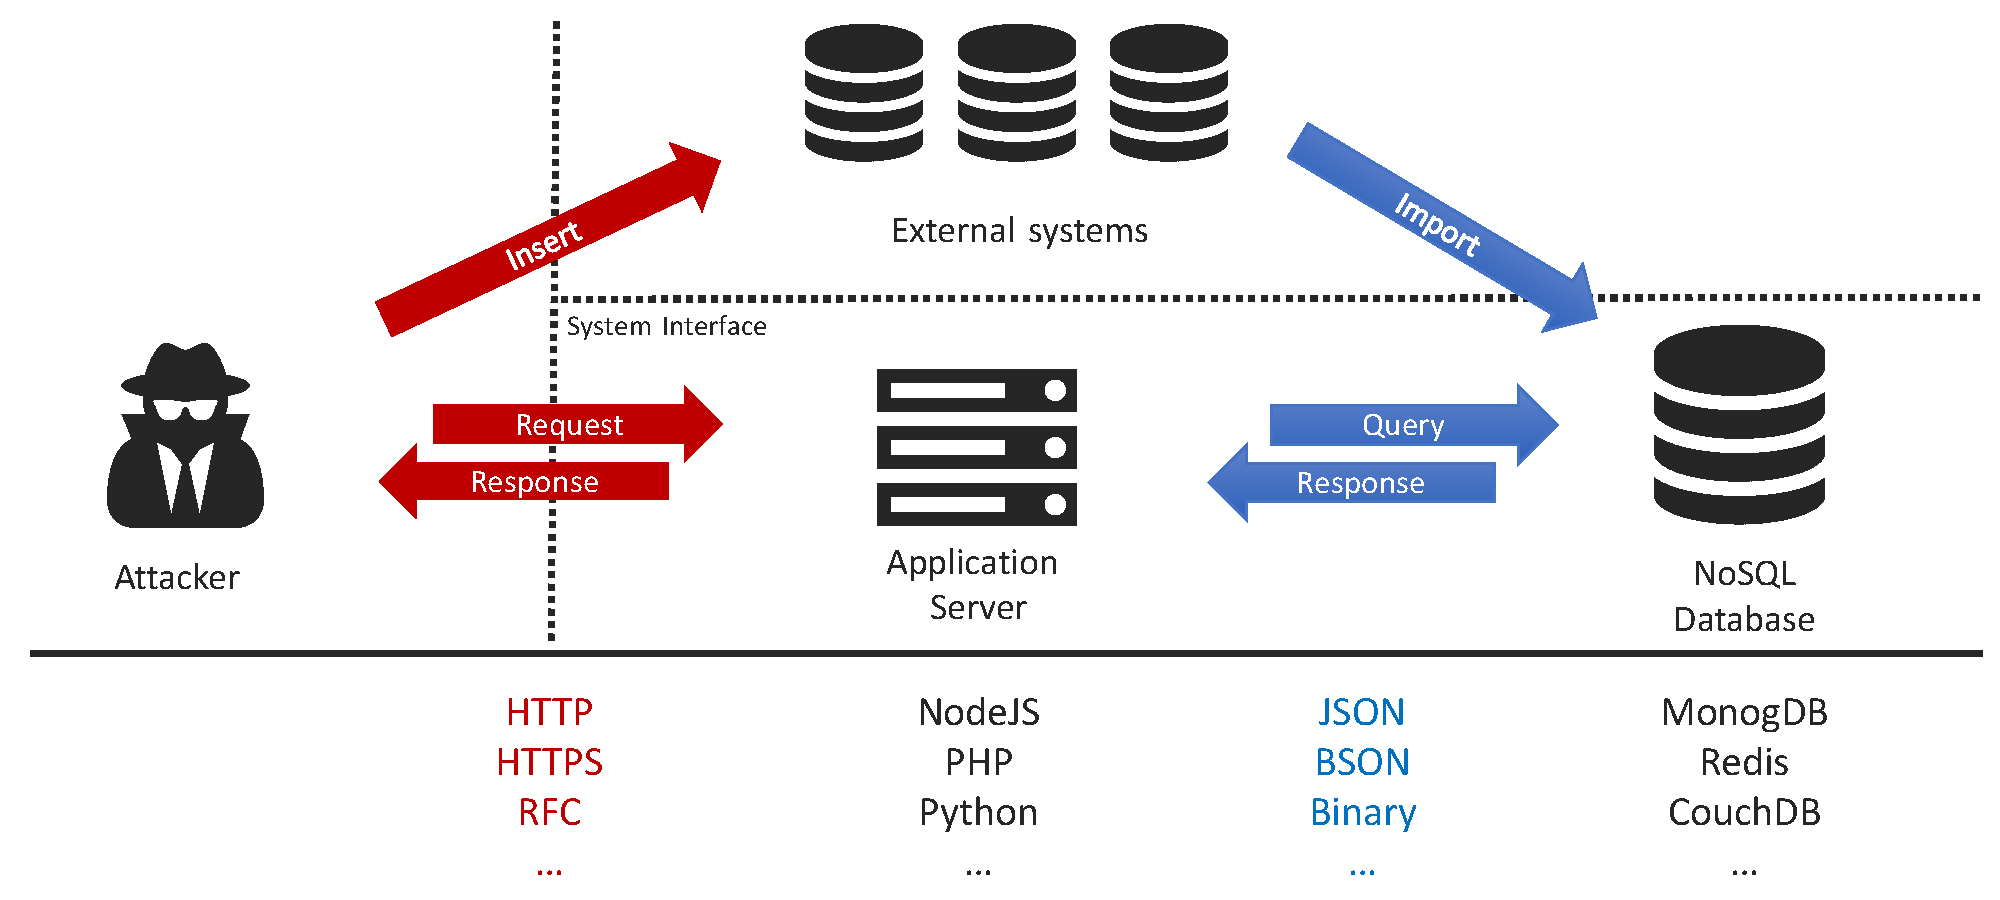
\includegraphics[width=1\linewidth]{Images/attacker_model_extended}
  \caption{Extended attacker model for NoSQL injection}
  \label{fig:extendedAttackerModel}
\end{figure}

% Objective

\subsection{Direct Attacker Model}

The deployment of RESTful interfaces allows a direct access from the client, omitting any application layer. Databases such as CouchDB explicitly refer to this architectural style for a simpler application design.

\begin{figure}[h]
\centering
  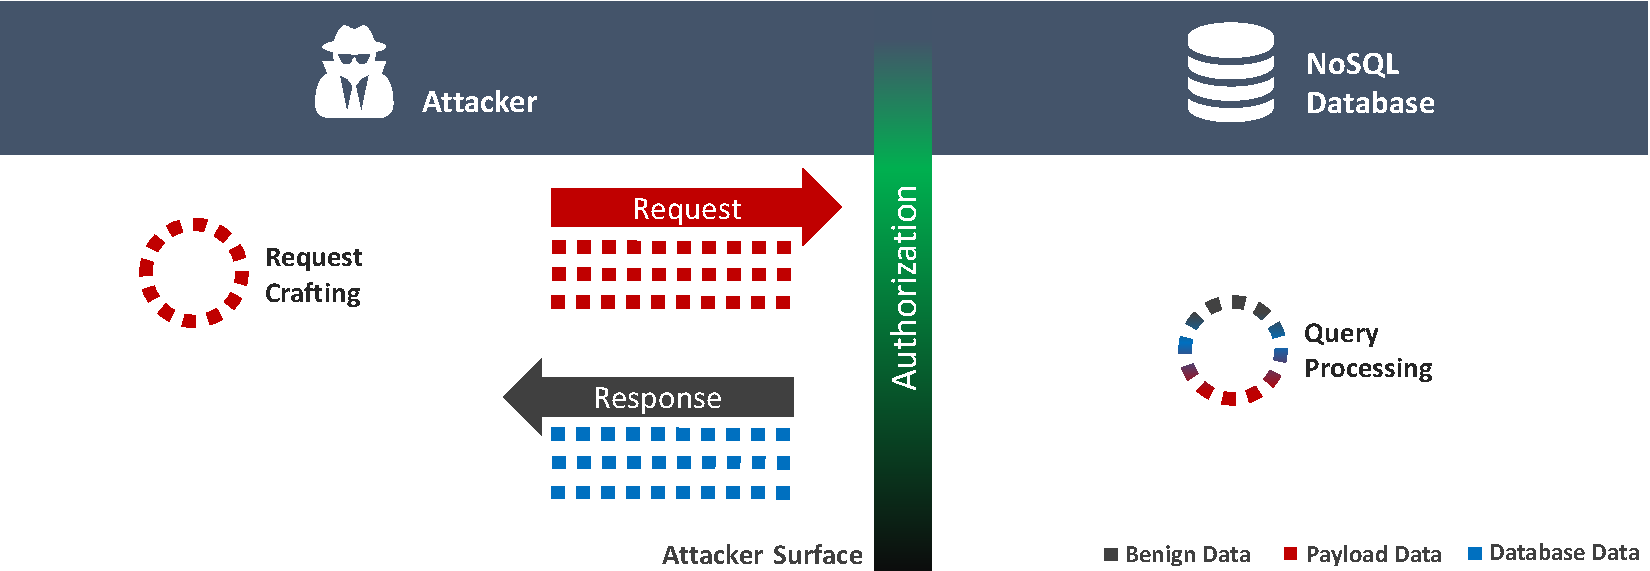
\includegraphics[width=1\linewidth]{Images/attacker_model_direct}
  \caption{Direct attacker model for NoSQL injection}
  \label{fig:extendedAttackerModel}
\end{figure}

% Objective


\section{Considered Technology Stack}
\subsection{Selected Databases}
\subsection{Selected Application Platforms}